\documentclass[a4paper, 12pt]{article}
\usepackage[brazil]{babel}
\usepackage[utf8]{inputenc}
\usepackage{graphicx}
\begin{document}

% espaços
Olá       Mundo!
Mesma linha.

Outro parágrafo.

A ativação de um neurônio:
\begin{equation}
y_i = \sum_{i=0}^{n} w_i \times x_i
\end{equation}

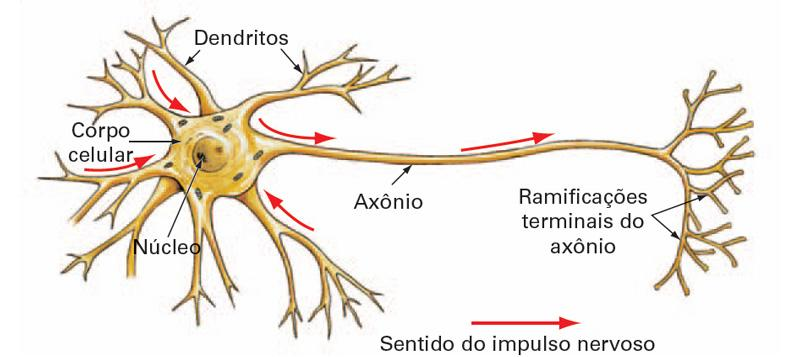
\includegraphics[scale=.5]{neuronio}
\end{document}
